\documentclass{beamer}
\usepackage[utf8]{inputenc}
\usepackage[english,russian]{babel}
\usepackage{amsmath,mathrsfs,mathtext}
\usepackage{graphicx,epsfig}
\usepackage{caption}
\usepackage{subfig}
\usetheme{Warsaw}%{Singapore}%{Warsaw}%{Warsaw}%{Darmstadt}
\usecolortheme{sidebartab}
%\definecolor{beamer@blendedblue}{RGB}{15,120,80}

\newcommand{\T}{^{\mathsf{T}}}
\DeclareMathOperator*{\argmax}{arg\,max}  % in your preamble
\DeclareMathOperator*{\argmin}{arg\,min}  % in your preamble 

\graphicspath{{../figures}, {../figures_delta}}

%\usepackage{biblatex}
\usepackage{hyperref}
\renewcommand{\thefootnote}{\arabic{footnote}}

%----------------------------------------------------------------------------------------------------------
\title[\hbox to 56mm{Восстановление снимков фМРТ \hfill\insertframenumber\,/\,\inserttotalframenumber}]
{Восстановление снимков фМРТ \\ по просматриваемому видеоряду}
\author[Н.\,С.~Киселев]{\large Никита Сергеевич Киселев}
\institute{\large
Московский физико-технический институт\par
(национальный исследовательский университет)}

\date{\footnotesize{\emph{Курс:} Автоматизация научных исследований\par (Моя первая научная статья)/Группа 003, весна 2023 \\
\par\emph{Эксперт:} А.\,В.~Грабовой
}}
%----------------------------------------------------------------------------------------------------------
\begin{document}
%----------------------------------------------------------------------------------------------------------
\begin{frame}
%\thispagestyle{empty}
\titlepage
\end{frame}
%-----------------------------------------------------------------------------------------------------
\begin{frame}{Цель исследования}
    \begin{block}{Проблема}
        Восстановление зависимости между показаниями датчиков фМРТ
        и восприятием внешнего мира человеком.
    \end{block}
    \begin{block}{Цель}
        Проверка линейной зависимости между последовательностью снимков фМРТ и видеорядом,
	    просматриваемым человеком.
    \end{block}
    \begin{block}{Решение}
        \begin{enumerate}
            \item Восстановление снимка фМРТ по
                    \begin{itemize}
                        \item одному изображению;
                        \item одному изображению и предыдущему снимку.
                    \end{itemize}
            \item Исследование свойств построенных методов и проверка гипотез.
        \end{enumerate}
    \end{block}
\end{frame}
%----------------------------------------------------------------------------------------------------------
\begin{frame}{Постановка задачи}
    Пусть задана частота кадров $\nu \in \mathbb{R}$ и продолжительность $t \in \mathbb{R}$ видеоряда. 
	Задан видеоряд
	\begin{equation*}
		\label{eq1}
		\mathbf{P} = [\mathbf{p}_1, \ldots, \mathbf{p}_{\nu \cdot t}], \quad\
		\mathbf{p}_i \in \mathbb{R}^{W_{\mathbf{P}} \times H_{\mathbf{P}} \times C_{\mathbf{P}}}.
	\end{equation*}

	Обозначим частоту снимков фМРТ $\mu \in \mathbb{R}$. Задана последовательность снимков 
	\begin{equation*}
		\label{eq2}
		\mathbf{S} = [\mathbf{s}_1, \ldots, \mathbf{s}_{\mu \cdot t}], \quad\
		\mathbf{s}_i \in \mathbb{R}^{W_{\mathbf{S}} \times H_{\mathbf{S}} \times D_{\mathbf{S}}}.
	\end{equation*}

	Необходимо построить отображение
    \begin{block}{}
        \begin{equation*}
            \label{eq3}
            g(\mathbf{p}_1, \ldots, \mathbf{p}_{k_i - \nu \cdot \Delta t}; \mathbf{s}_1, \ldots, \mathbf{s}_{i-1}) = \mathbf{s}_i,
        \end{equation*}
        \begin{equation*}
            \label{eq4}
            i = 1, \ldots, \mu t, \qquad k_i = \dfrac{i \cdot \nu}{\mu}.
        \end{equation*}
    \end{block}
\end{frame}
%----------------------------------------------------------------------------------------------------------
\begin{frame}{Базовая модель}
    Каждый снимок зависит только от одного изображения.
	\begin{equation*}
		\label{eq5}
		g(\mathbf{p}_{k_i - \nu \cdot \Delta t}) = \mathbf{s}_i, \ i = 1, \ldots, \mu t.
	\end{equation*}
    Число снимков в выборке $N = N_{\mathbf{S}} - \mu \Delta t$.
    \begin{block}{Модель и функция потерь}
        \begin{equation*}
            \label{eq7}
            f_{ijk}(\mathbf{x}, \mathbf{w}_{ijk}) = \langle \mathbf{x}, \mathbf{w}_{ijk} \rangle
        \end{equation*}
        \begin{equation*}
            \label{eq8}
            \mathcal{L}_{ijk}(\mathbf{w}_{ijk}, \Delta t) = \sum\limits_{\ell = 1}^{N_{\mathbf{S}} - \mu \Delta t} \big(f_{ijk}(\mathbf{x}_{\ell}, \mathbf{w}_{ijk}) - v^{\ell}_{ijk}\big)^2
        \end{equation*}
        \begin{itemize}
            \item $\mathbf{x}_{\ell} = [x^{\ell}_1, \ldots, x^{\ell}_{d}]\T \in \mathbb{R}^{d}$~--- признаки изображения;
            \item $\mathbf{w}_{ijk} = [w^{ijk}_1, \ldots, w^{ijk}_{d}]\T \in \mathbb{R}^{d}$~--- вектор параметров;
            \item $\mathbf{s}_{\ell} = [v^{\ell}_{ijk}] \in \mathbb{R}^{W_{\mathbf{S}} \times H_{\mathbf{S}} \times D_{\mathbf{S}}}$~--- снимок фМРТ.
        \end{itemize}
    \end{block}
\end{frame}
%----------------------------------------------------------------------------------------------------------
\begin{frame}{Решение в базовой модели}
    \begin{equation*}
		\label{eq9}
		\hat{\mathbf{w}}_{ijk} = \argmin_{\mathbf{w}_{ijk}} \mathcal{L}_{ijk}(\mathbf{w}_{ijk}, \Delta t).
	\end{equation*}

    \begin{block}{Метод наименьших квадратов}
        \begin{equation*}
            \label{eq12}
            \hat{\mathbf{w}}_{ijk} = (\mathbf{X}\T \mathbf{X})^{-1} \mathbf{X}\T \mathbf{v}_{ijk} = \mathbf{X}^{+} \mathbf{v}_{ijk},
	    \end{equation*}
        \begin{itemize}
            \item $\mathbf{X} = [\mathbf{x}_1\T, \ldots, \mathbf{x}_N\T]\T = [x^i_j] \in \mathbb{R}^{N \times d}$~--- матрица плана;
            \item $\mathbf{v}_{ijk} = [v^1_{ijk}, \ldots, v^N_{ijk}]\T \in \mathbb{R}^N$~--- воксель в разных снимках.
        \end{itemize}
    \end{block}
\end{frame}
%----------------------------------------------------------------------------------------------------------
\begin{frame}{Основная модель}
    Каждый снимок зависит только от одного изображения и предыдущего снимка.
	\begin{equation*}
		\label{eq15}
		g(\mathbf{p}_{k_i - \nu \Delta t}; \mathbf{s}_{i-1}) = \mathbf{s}_i, \ i = 1, \ldots, \mu t.
	\end{equation*}
    Число снимков в выборке $N = N_{\mathbf{S}} - \mu \Delta t - 1$.
    \begin{block}{Модель и функция потерь}
        \begin{equation*}
            \label{eq15}
            f_{ijk}(\mathbf{x}, \mathbf{w}_{ijk}) = \langle \mathbf{x}, \mathbf{w}_{ijk} \rangle
        \end{equation*}
        \begin{equation*}
            \label{eq16}
            \mathcal{L}_{ijk}(\mathbf{w}_{ijk}, \Delta t) = \sum\limits_{\ell = 1}^{N_{\mathbf{S}} - \mu \Delta t - 1} \big(f_{ijk}(\mathbf{x}_{\ell}, \mathbf{w}_{ijk}) - (v^{\ell + 1}_{ijk} - v^{\ell}_{ijk})\big)^2 + \alpha \| \mathbf{w}_{ijk} \|_2^2
        \end{equation*}
        \begin{itemize}
            \item $\mathbf{x}_{\ell} = [x^{\ell}_1, \ldots, x^{\ell}_{d}]\T \in \mathbb{R}^{d}$~--- признаки изображения;
            \item $\mathbf{w}_{ijk} = [w^{ijk}_1, \ldots, w^{ijk}_{d}]\T \in \mathbb{R}^{d}$~--- вектор параметров;
            \item $\mathbf{s}_{\ell} = [v^{\ell}_{ijk}] \in \mathbb{R}^{W_{\mathbf{S}} \times H_{\mathbf{S}} \times D_{\mathbf{S}}}$~--- снимок фМРТ.
        \end{itemize}
    \end{block}
\end{frame}
%----------------------------------------------------------------------------------------------------------
\begin{frame}{Решение в основной модели}
    \begin{equation*}
		\label{eq17}
		\hat{\mathbf{w}}_{ijk} = \argmin_{\mathbf{w}_{ijk}} \mathcal{L}_{ijk}(\mathbf{w}_{ijk}, \Delta t).
	\end{equation*}

    \begin{block}{Метод наименьших квадратов}
        \begin{equation*}
            \label{eq20}
            \hat{\mathbf{w}}_{ijk} = (\mathbf{X}\T \mathbf{X} + \alpha \mathbf{I})^{-1} \mathbf{X}\T \mathbf{\Delta v}_{ijk}.
        \end{equation*}
        \begin{itemize}
            \item $\mathbf{X} = [\mathbf{x}_2\T, \ldots, \mathbf{x}_N\T]\T = [x^i_j] \in \mathbb{R}^{(N-1) \times d}$~--- матрица плана;
            \item $\mathbf{I}$~--- единичная матрица;
            \item $\mathbf{\Delta v}_{ijk} = [v^2_{ijk} - v^1_{ijk}, \ldots, v^N_{ijk} - v^{N-1}_{ijk}]\T \in \mathbb{R}^{N-1}$~--- разности вокселей двух последовательных снимков.
        \end{itemize}
    \end{block}
\end{frame}
%----------------------------------------------------------------------------------------------------------
\begin{frame}{Вычислительный эксперимент}
    \begin{block}{Цель}
        \begin{enumerate}
            \item Проверка работоспособности предложенных методов.
            \item Исследование зависимости качества восстановления от гиперпараметра $\Delta t$.
            \item Проверка гипотез:
                    \begin{itemize}
                        \item линейная зависимость между данными;
                        \item взаимосвязь снимков в последовательности;
                        \item инвариантность весов модели относительно человека.
                    \end{itemize}
        \end{enumerate}
    \end{block}
    \begin{block}{Данные}
        Реальное фМРТ-обследование\footnotemark 30 испытуемых разного пола и возраста.
        Каждый из них просматривал короткий аудиовизуальный фильм.
        Продолжительность фильма $t = 390$~с, частота кадров $\nu = 25$.
        Частота снимков $\mu = 1.64$.
    \end{block}
    \footnotetext[1]{\href{https://doi.org/10.1038/s41597-022-01173-0}{Ссылка на датасет}}
\end{frame}
%----------------------------------------------------------------------------------------------------------
\begin{frame}{Базовый метод~--- зависимость от гиперпараметра}
    Зависимость метрики MSE от гиперпараметра $\Delta t$ для фиксированного испытуемого.
    Использовалось предварительное 8-кратное сжатие снимка.
    \begin{figure}
        \centering
        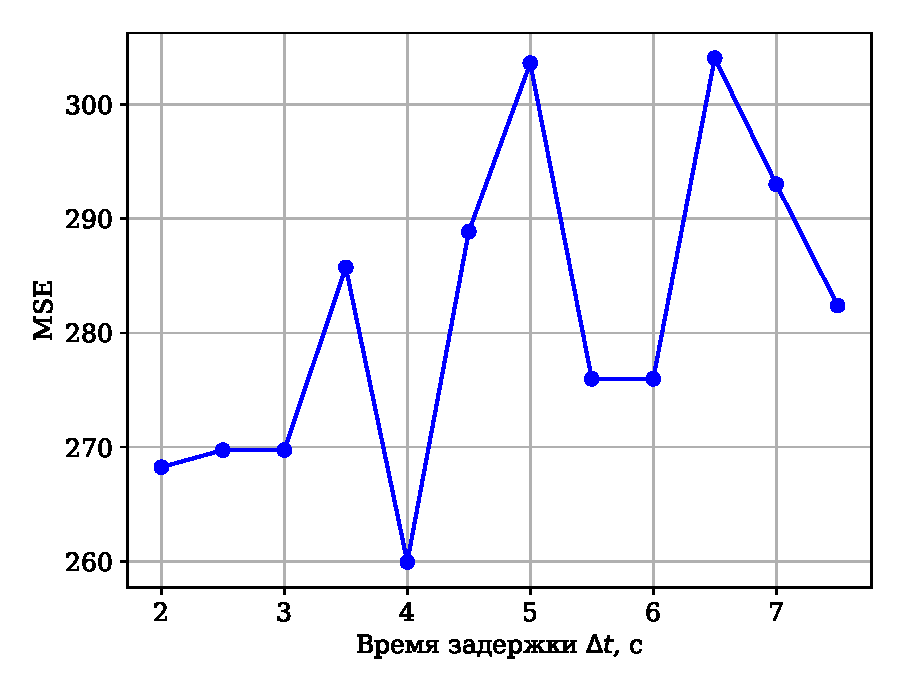
\includegraphics[width = 0.7\textwidth]{MSE_dt.eps}
    \end{figure}
    Наблюдается минимум MSE при $\Delta t = 4 \text{ с}$.
\end{frame}
%----------------------------------------------------------------------------------------------------------
\begin{frame}{Базовый метод~--- восстановленный снимок}
    Срезы истинного и восстановленного снимков из тестовой выборки.
    Использовалось предварительное 4-кратное сжатие снимка.
    Из восстановленного снимка отброшены нефизичные значения.
    Далее применен фильтр Гаусса.
    \begin{figure}[h!]
		\centering
		\subfloat[Истинный]{\label{fig:1a}{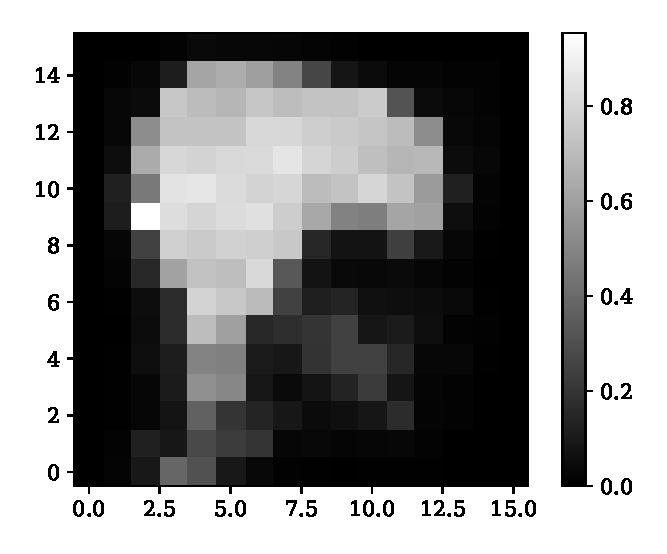
\includegraphics[width=0.33\textwidth]{sub-04-4-4-5-_-_-orig.eps}}}
		\hfill
		\subfloat[Восстановленный]{\label{fig:1b}{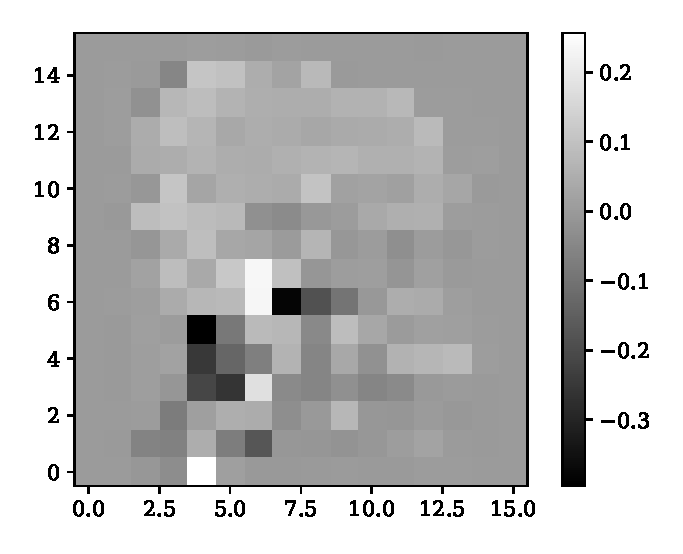
\includegraphics[width=0.33\textwidth]{sub-04-4-4-5-_-_-pred.eps}}}
		\hfill
		\subfloat[Обработанный]{\label{fig:1c}{\includegraphics[width=0.33\textwidth]{sub-04-4-4-5-_-_-pred-pg.eps}}}
		\label{fig:1}
	\end{figure}
    В рассматриваемом методе не учитывается взаимосвязь соседних снимков и вокселей.
    Наблюдаются большие выбросы в восстановленных значениях.
    Однако видны границы активных областей.
\end{frame}
%----------------------------------------------------------------------------------------------------------
\begin{frame}{Основной метод~--- зависимость от гиперпараметра}
    Зависимость метрики MSE от гиперпараметра $\Delta t$.
    Использовалось предварительное 8-кратное сжатие снимка.
    Производилось усреднение по испытуемым.
	Обозначены границы среднеквадратичного отклонения.
    \begin{figure}[h!]
		\centering
		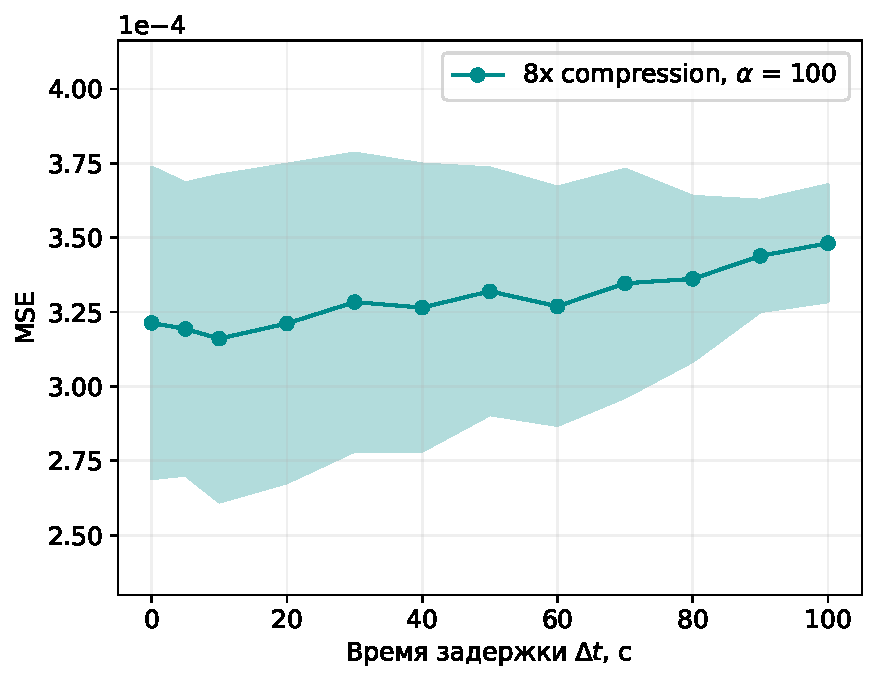
\includegraphics[width=0.65\textwidth]{subs_delta_MSE_dt.pdf}
		\label{fig:3}
	\end{figure}
    Наблюдается минимум MSE при $\Delta t = 10 \text{ с}$.
\end{frame}
%----------------------------------------------------------------------------------------------------------
\begin{frame}{Основной метод~--- восстановленный снимок}
    Срезы истинного и восстановленного снимков из тестовой выборки.
    Можно наблюдать разность между ними.
    \begin{figure}[h!]
		\centering
		\subfloat[Истинный]{\label{fig:4a}{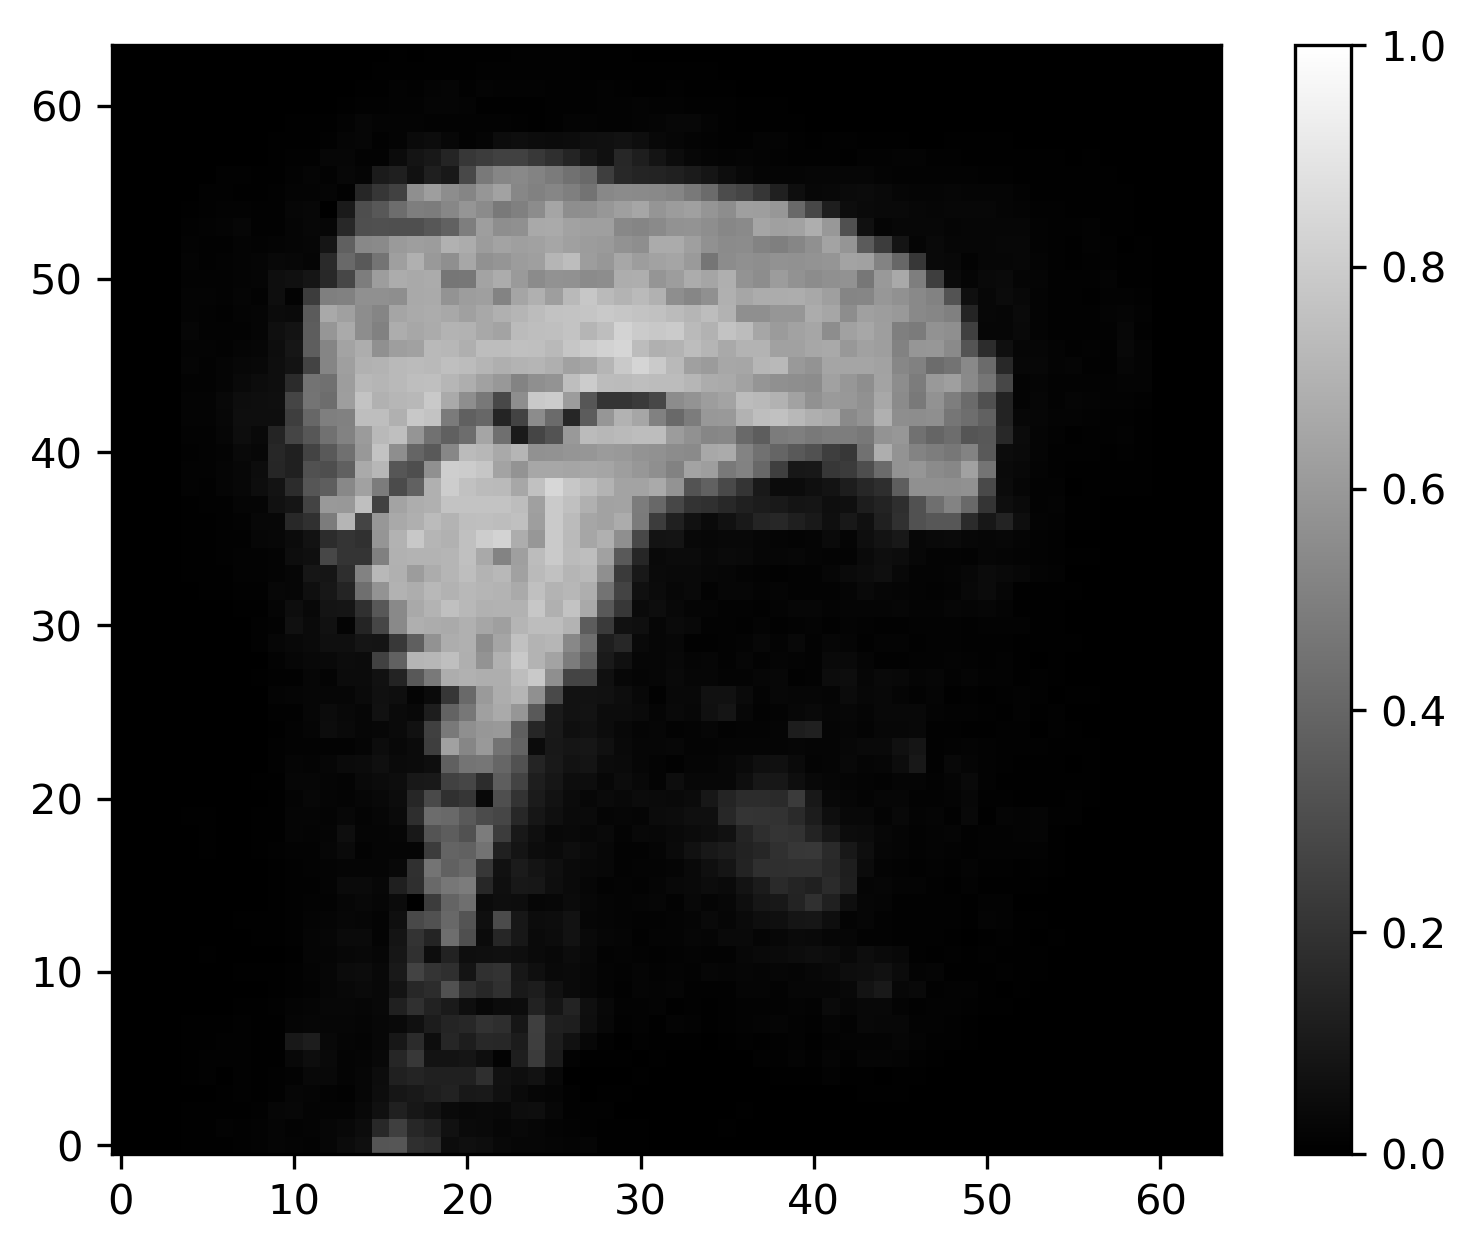
\includegraphics[width=0.33\textwidth]{sub-04-5-1-1000/sub-04-5-1-1000-100-20-_-_-test.png}}}
		\hfill
		\subfloat[Восстановленный]{\label{fig:4b}{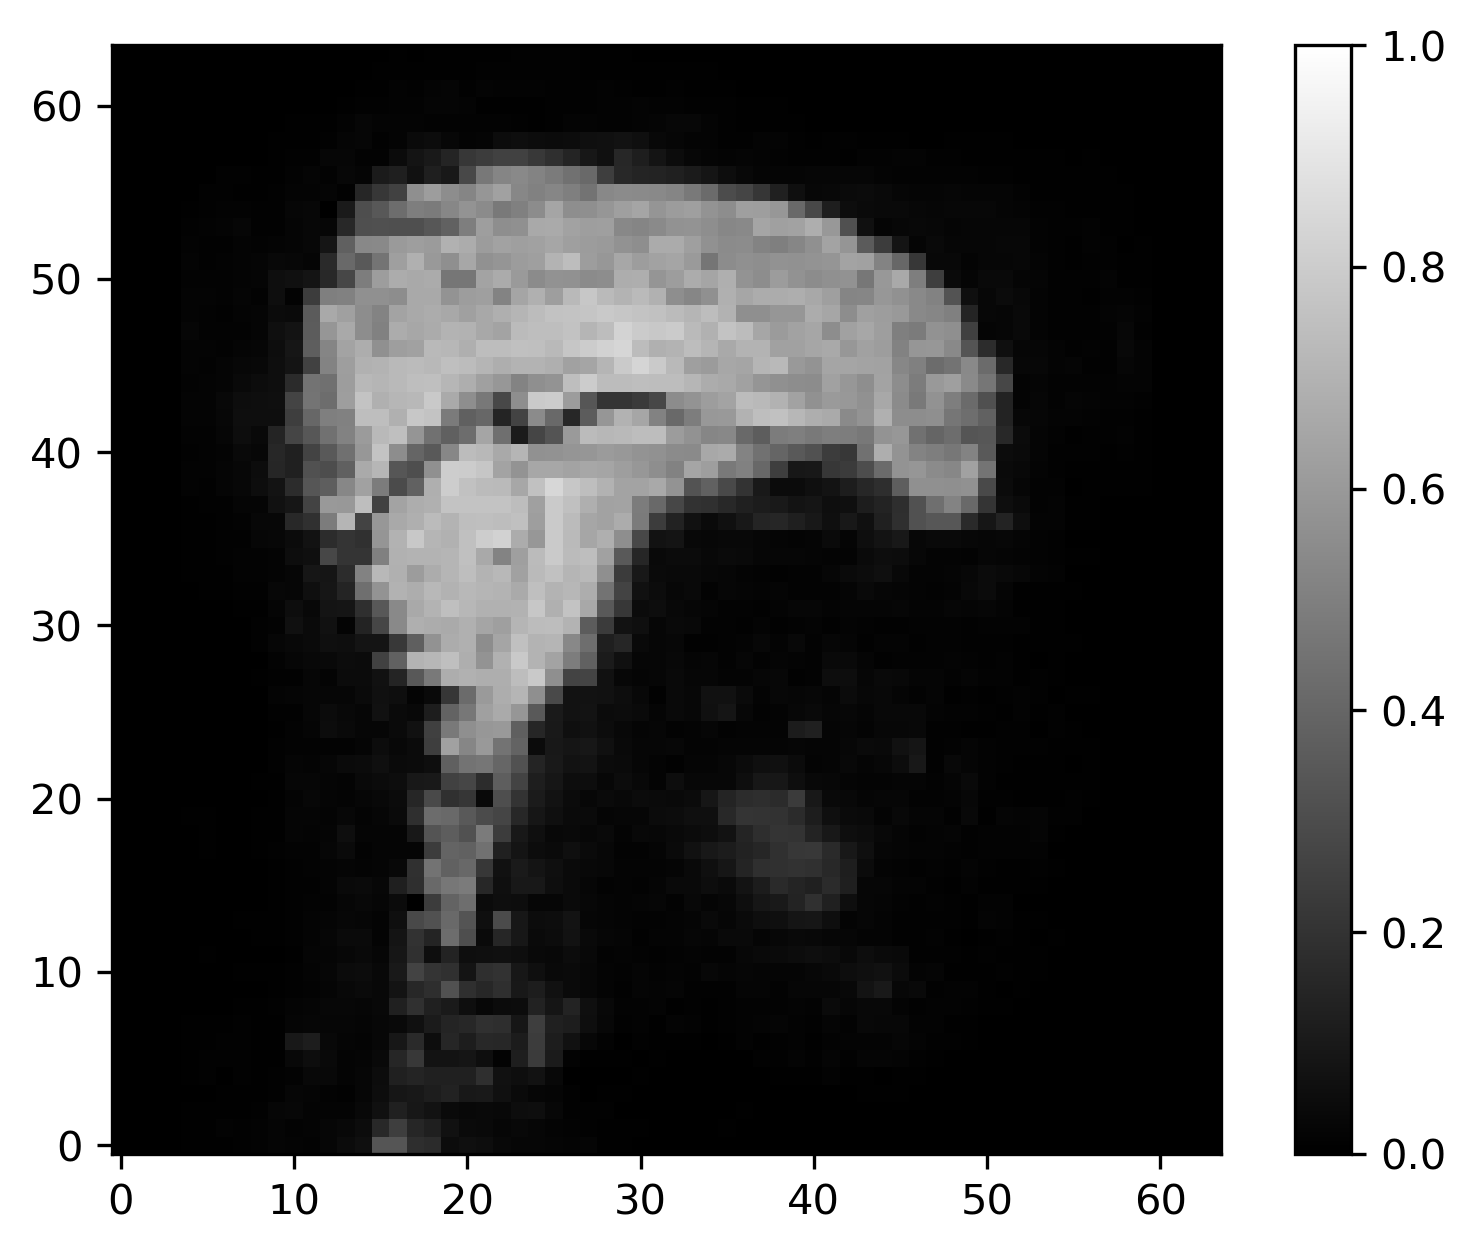
\includegraphics[width=0.33\textwidth]{sub-04-5-1-1000/sub-04-5-1-1000-100-20-_-_-predicted.png}}}
		\hfill
		\subfloat[Разность]{\label{fig:4c}{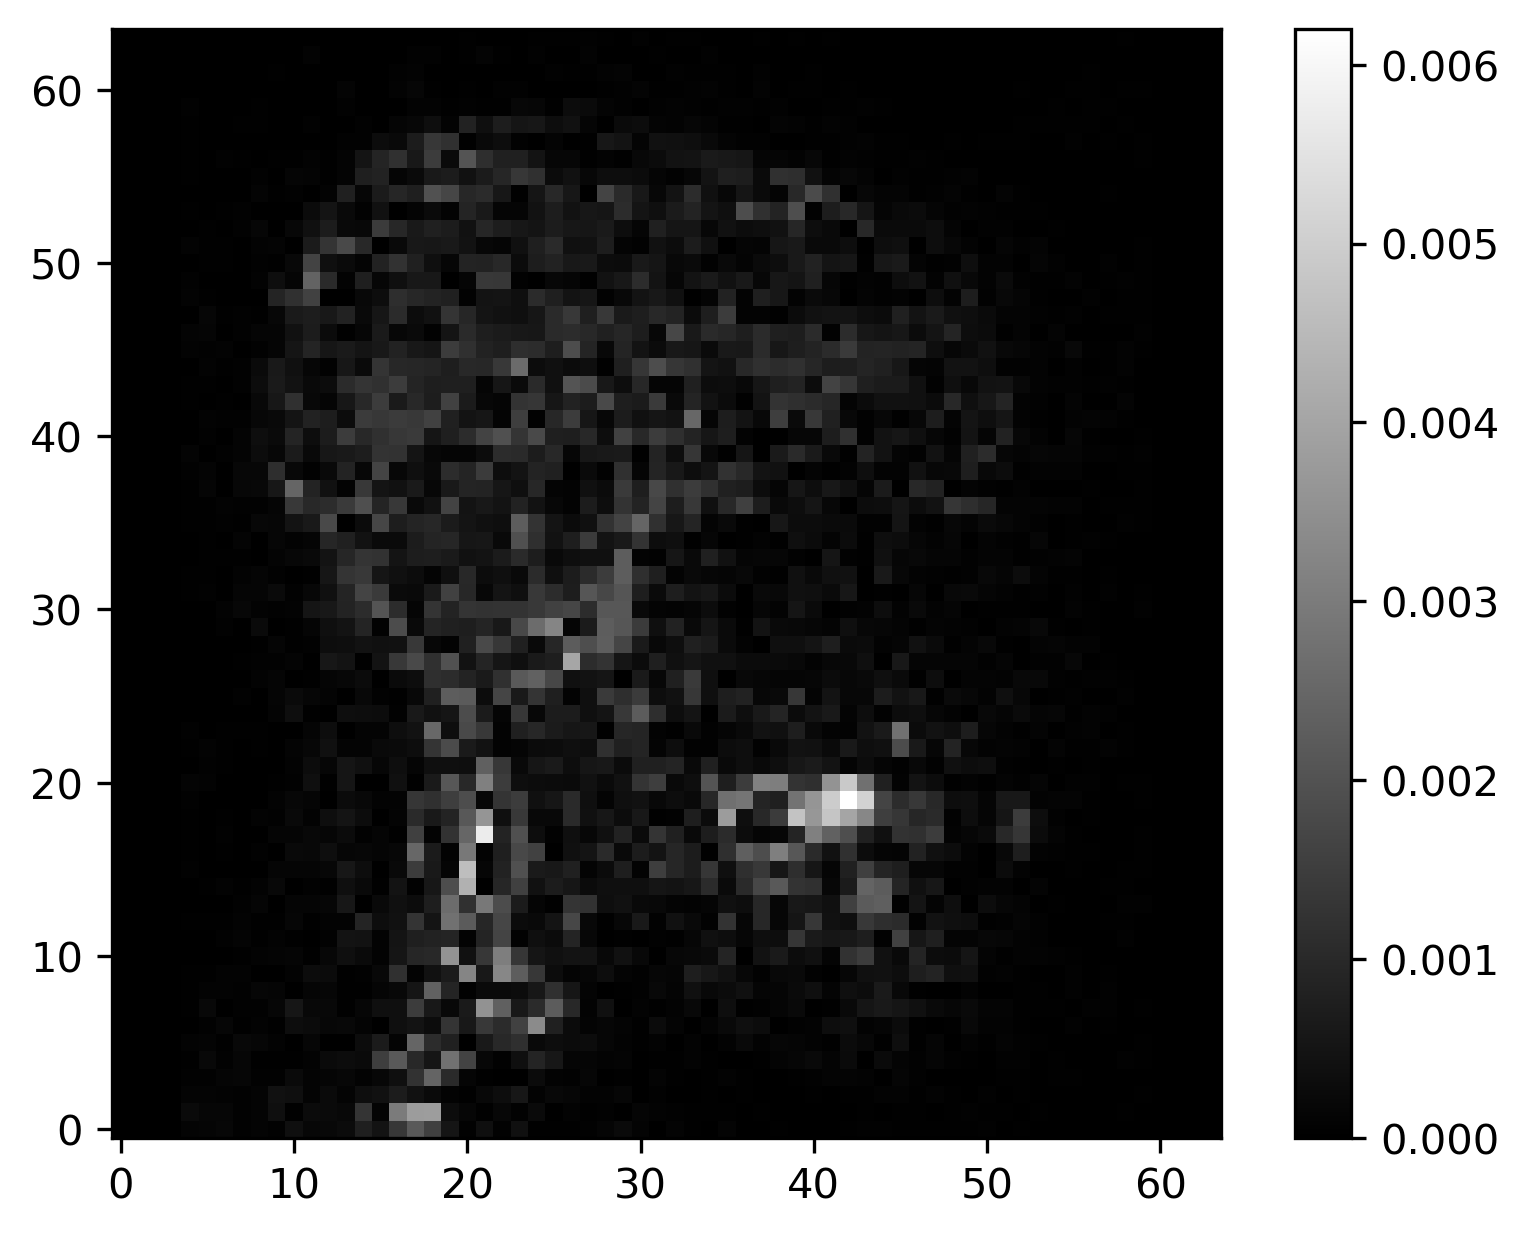
\includegraphics[width=0.33\textwidth]{sub-04-5-1-1000/sub-04-5-1-1000-100-20-_-_-difference.png}}}
		\label{fig:4}
	\end{figure}
    Качество восстановления значительно улучшилось по сравнению с базовым методом.
\end{frame}
%----------------------------------------------------------------------------------------------------------
\begin{frame}{Основной метод~--- зависимость от $\alpha$}
    Зависимость метрики MSE от коэффициента регуляризации $\alpha$.
    Рассматривались коэффициенты сжатия 1, 2, 4 и 8.
    Производилось усреднение по испытуемым.
	Обозначены границы среднеквадратичного отклонения.
    \begin{figure}[h!]
		\centering
		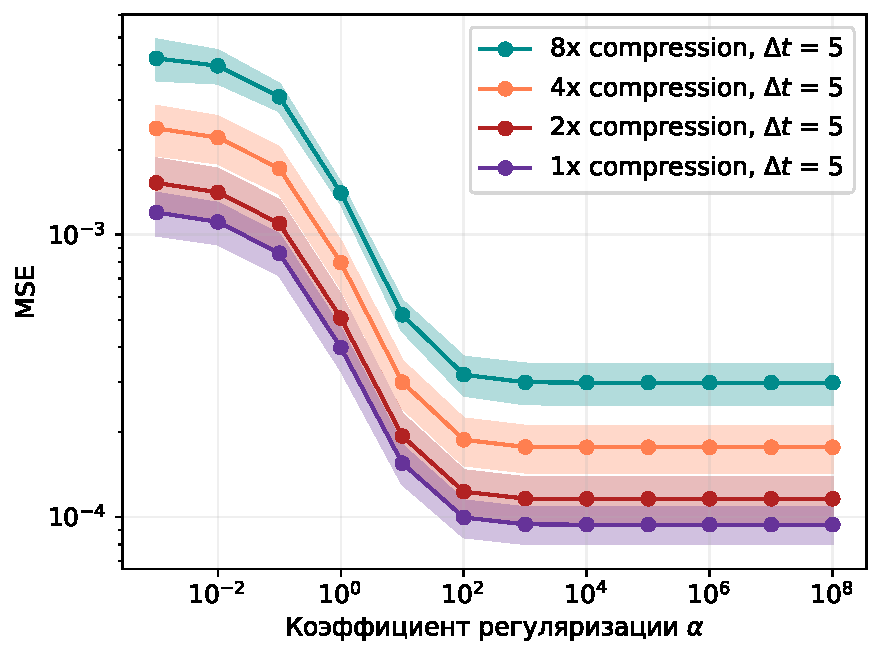
\includegraphics[width=0.65\textwidth]{subs_MSE_alpha.pdf}
		\label{fig:5}
	\end{figure}
    Оптимальное значение коэффициента $\alpha \approx 100$.
\end{frame}
%----------------------------------------------------------------------------------------------------------
\begin{frame}{Основной метод~--- распределение весов}
    График распределения значений компонент вектора весов модели.
    Производилось усреднение по всем вокселям фиксированного снимка.
    \begin{figure}[h!]
		\centering
		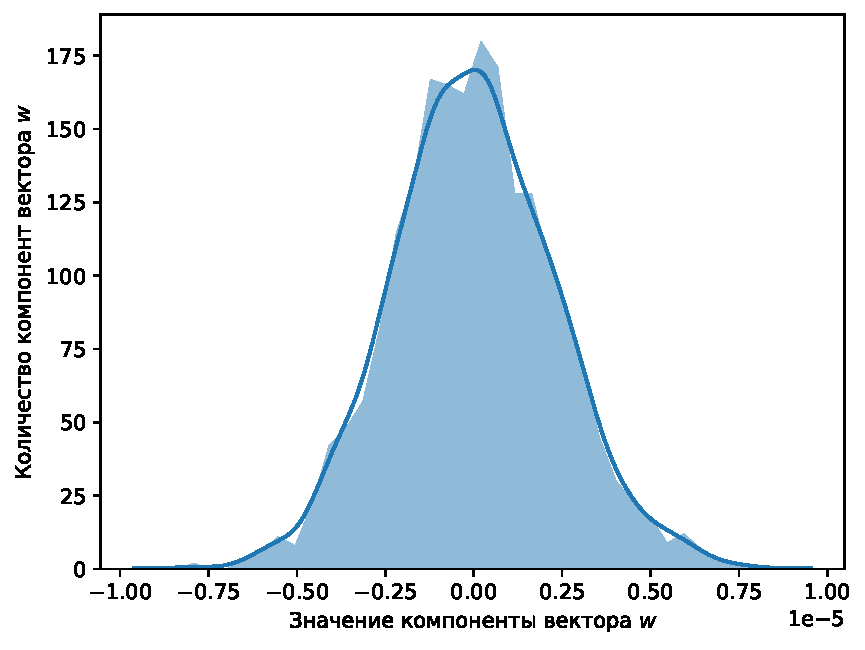
\includegraphics[width=0.65\textwidth]{mean_weight_distribution.pdf}
		\label{fig:6}
	\end{figure}
    Аппроксимация распределения схожа с плотностью нормального распределения.
\end{frame}
%----------------------------------------------------------------------------------------------------------
\begin{frame}{Основной метод~--- инвариантность весов}
    Проведена проверка гипотезы инвариантности весов модели относительно человека:
	можно ли восстановление снимка фМРТ одного испытуемого, используя
	матрицу весов другого. Использовалась метрика MSE на тестовой выборке.
    \begin{table}[h!]
		\centering
		\begin{tabular}{|c|c|c|}
			\hline
			Матрица весов	&	Истинная	&	Подмешанная \\ \hline \hline
			MSE		& 	$1.02 \cdot 10^{-4}$	 &		$1.05 \cdot 10^{-4}$ \\ \hline
		\end{tabular}
		\label{table:1}
	\end{table}
\end{frame}
%----------------------------------------------------------------------------------------------------------
\begin{frame}{Основной метод~--- случайный шум}
    Рассмотрено качество работы метода на случайном шуме. В качестве матрицы $\mathbf{X}$
	взята матрица случайных чисел из $[0, 1)$. Ниже приведены срезы последнего снимка, восстановленного
    последовательно по всем предсказанным изменениям, и значения метрики MSE.
	\begin{figure}[h!]
		\centering
		\subfloat[Истинный]{\label{fig:8a}{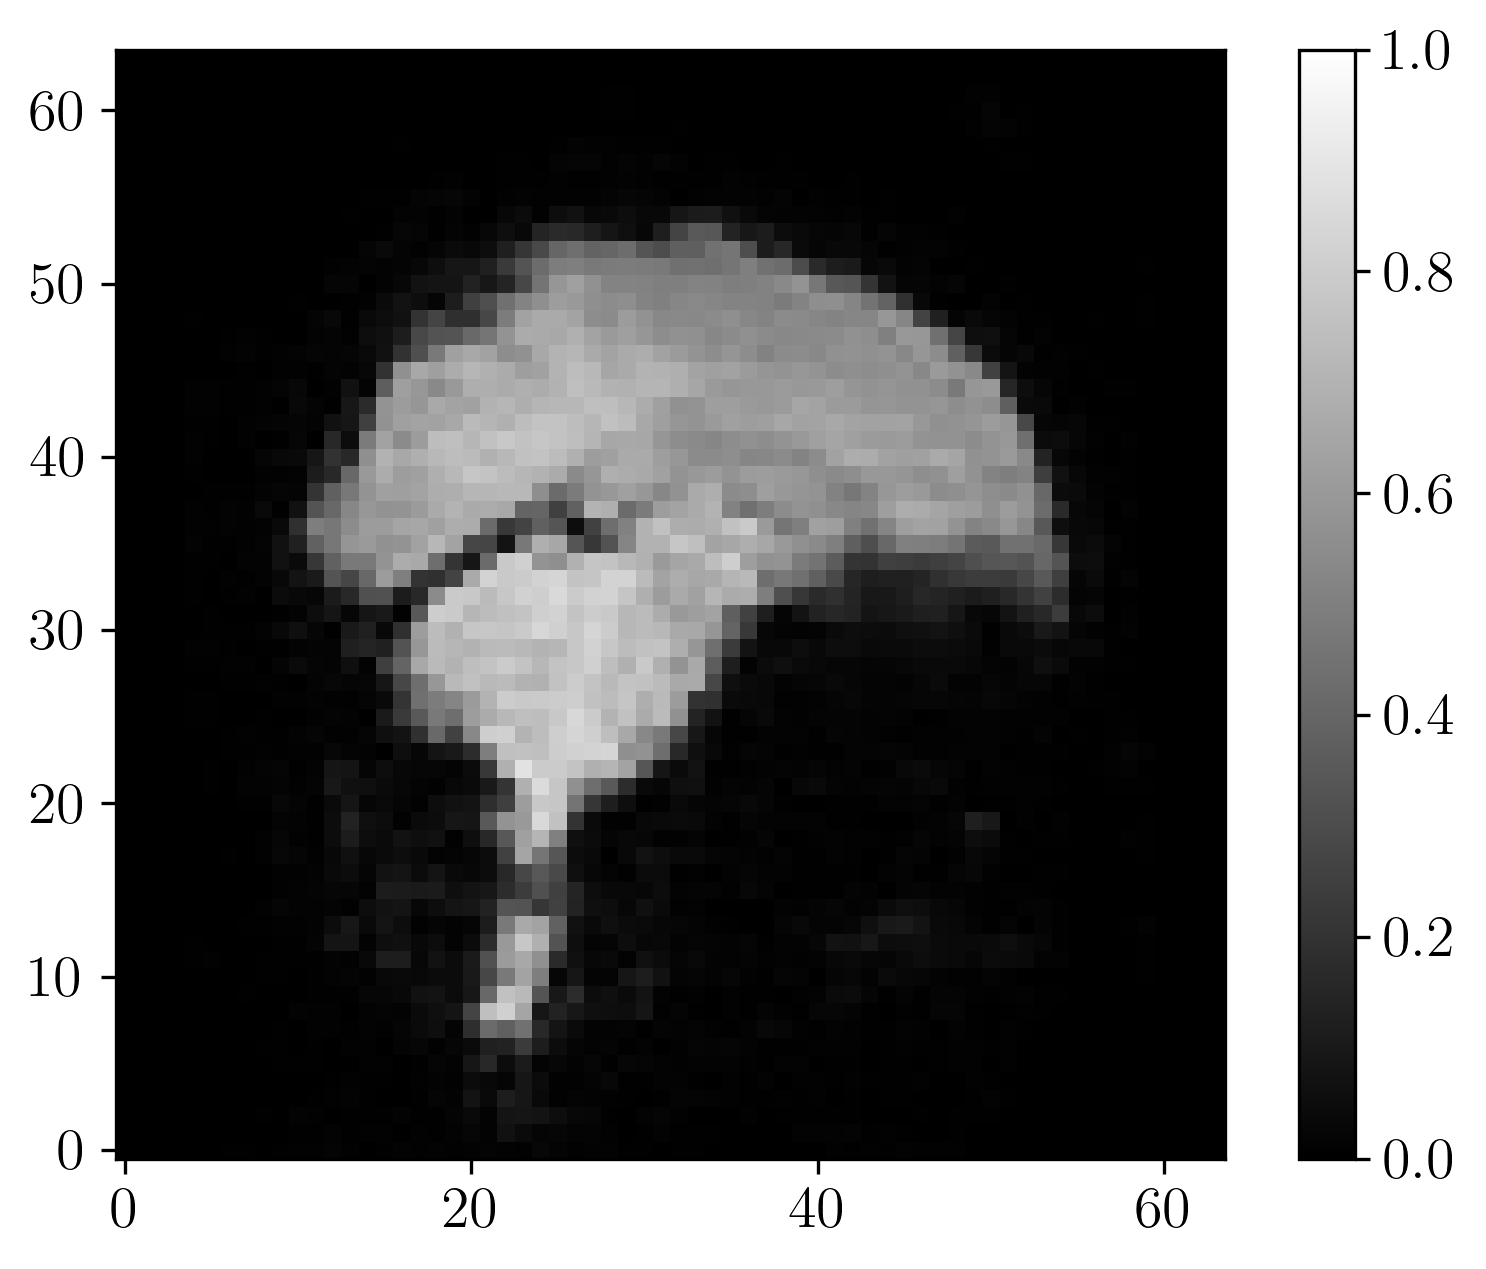
\includegraphics[width=0.33\textwidth]{sub-35-5-1-1000/noised/sub-35-5-1-1000--1-20-_-_-recovered-test.png}}}
		\hfill
		\subfloat[Восстановленный]{\label{fig:8b}{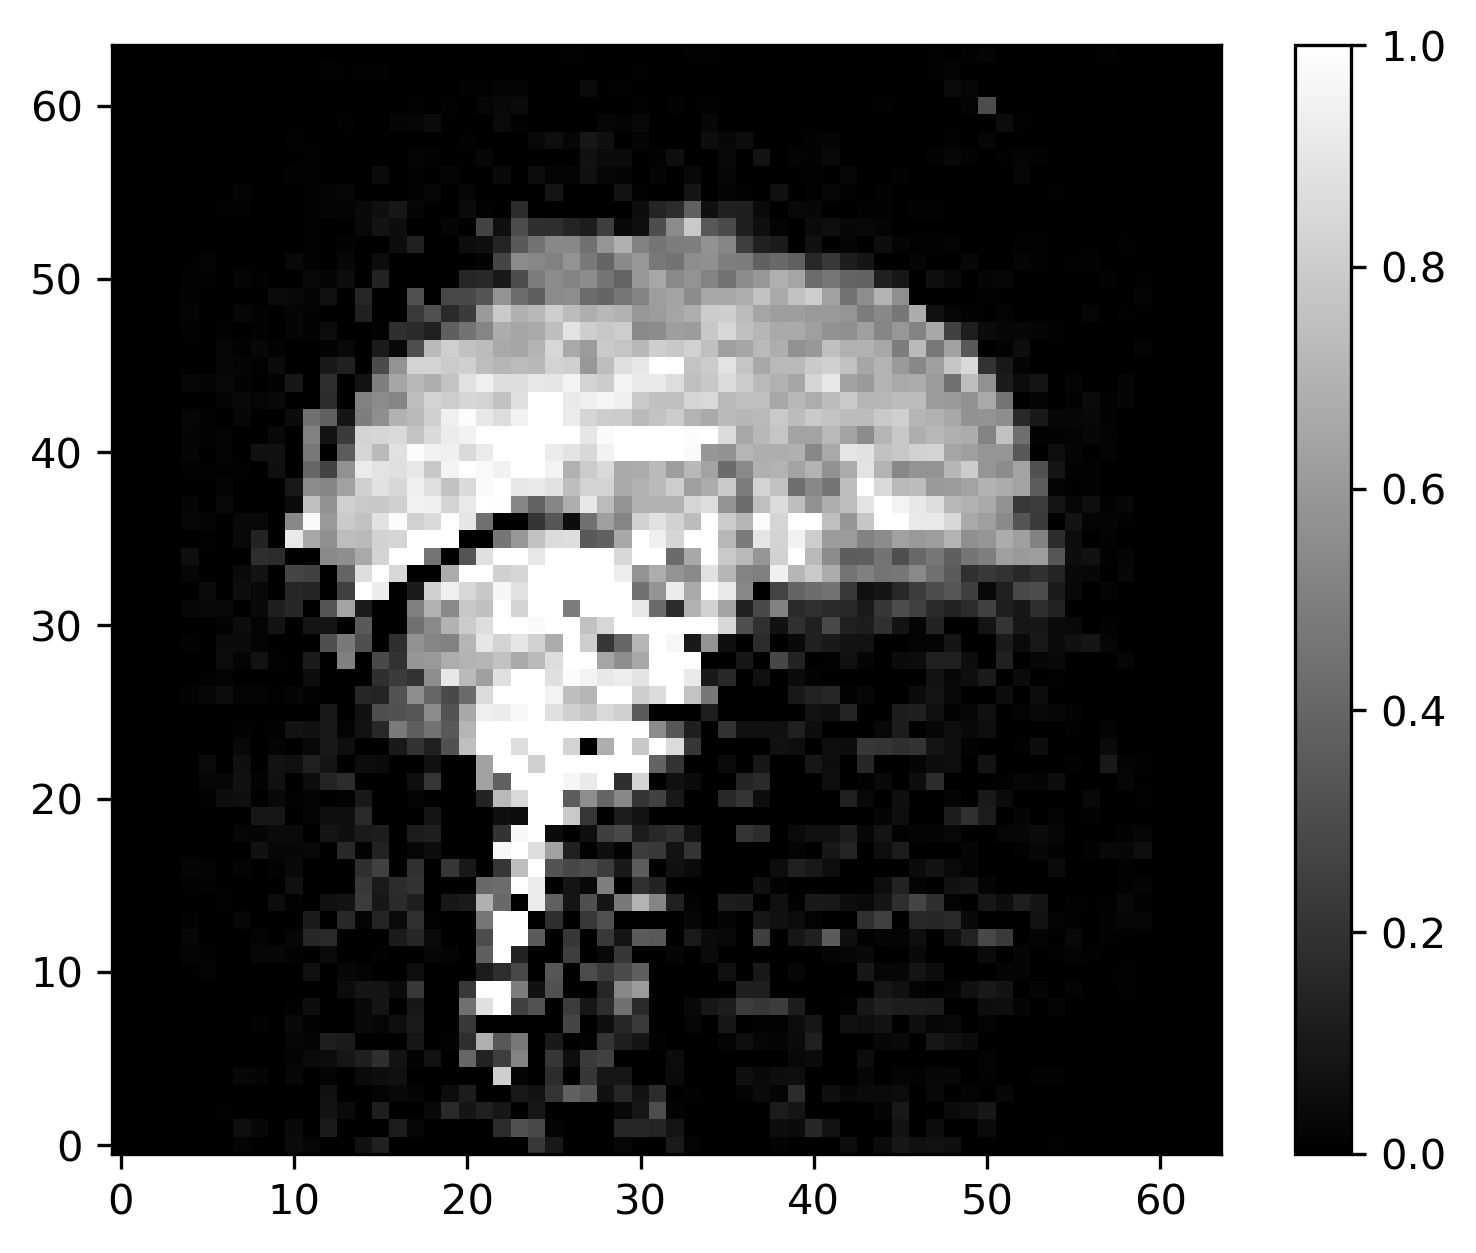
\includegraphics[width=0.33\textwidth]{sub-35-5-1-1000/noised/sub-35-5-1-1000--1-20-_-_-recovered-predicted.png}}}
		\hfill
		\subfloat[Разность]{\label{fig:8c}{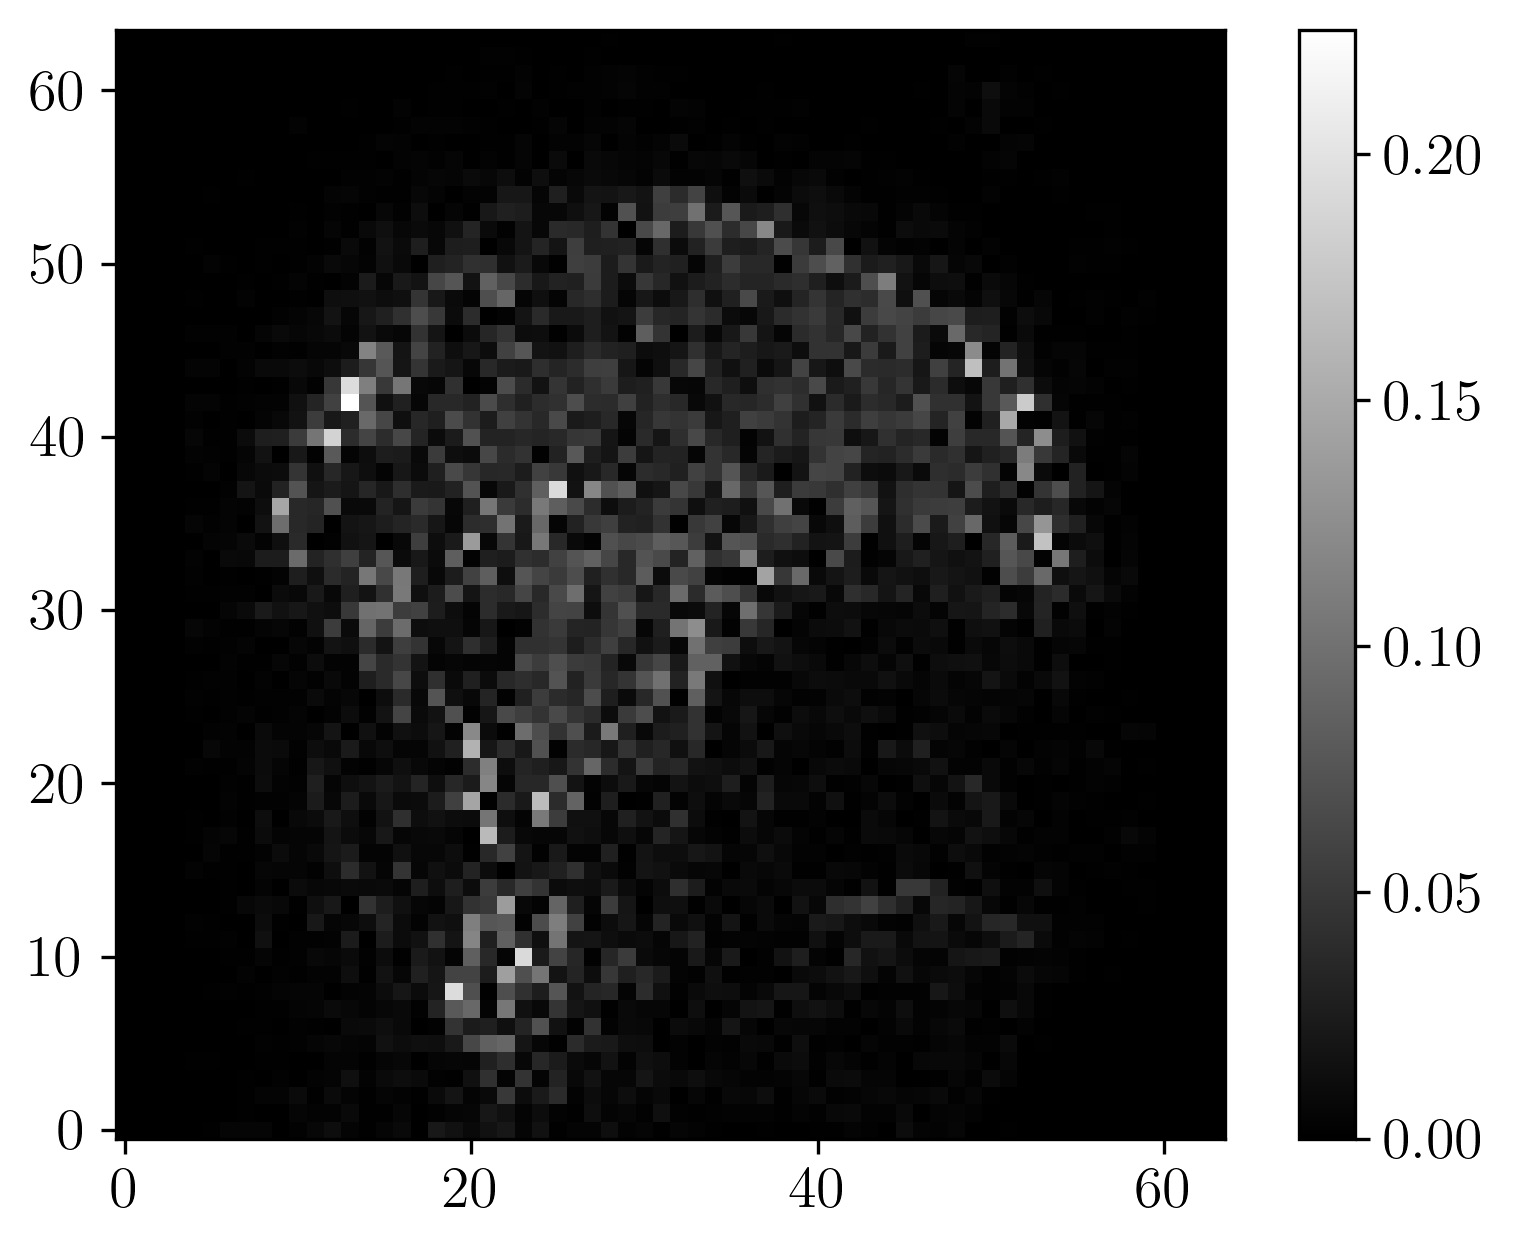
\includegraphics[width=0.33\textwidth]{sub-35-5-1-1000/noised/sub-35-5-1-1000--1-20-_-_-recovered-difference.png}}}
		\label{fig:8}
	\end{figure}
    \begin{table}[h!]
		\centering
		\begin{tabular}{|c|c|c|}
			\hline
			Выборка	&	Истинная	&	Случайный шум \\ \hline \hline
			MSE		& 	$2 \cdot 10^{-3}$	 &		$10^{-1}$ \\ \hline
		\end{tabular}
		\label{table:2}
	\end{table}    
\end{frame}
%----------------------------------------------------------------------------------------------------------
\begin{frame}{Заключение}
    \begin{itemize}
        \item Построены базовый и основной методы восстановления снимков фМРТ по видеоряду, просматриваемому
        человеком.
        \item Оба метода показывают справедливость гипотезы о линейной зависимости между данными.
        \item Качество работы основного метода значительно лучше.
        \item Это подтверждает гипотезу о взаимосвязи снимков в последовательности.
        \item Проверена гипотеза инвариантности весов модели относительно человека.
    \end{itemize}
\end{frame}
%----------------------------------------------------------------------------------------------------------
\end{document} 